%grundlagen.tex

\chapter{Grundlagen}
\label{chapter:gru}

\section{Chromatographie}

Die Chromatographie ist ein Verfahren zur Auftrennung von Stoffgemischen. 
Die Auftrennung erfolgt dabei zwischen zwei sogenannten Phasen, der stationären und der mobilen Phase, welche sich in unterschiedlichen Aggregatzuständen befinden und untereinander nicht mischen. 

Es existieren zum einen die Flüssigchromatographie (LC, engl. Liquid Chromatography),
\todo{Muss englische Worterklärung kursiv oä?}
bei der die mobile Phase eine Flüssigkeit ist und die stationäre Phase ein Feststoff. Bei der Gaschromatographie (GC) ist die mobile Phase ein Gas und es wird zusätzlich nach der stationären Phase unterschieden. Ist diese ein Feststoff, so spricht man von gepackten Säulen. Bei der Kapillartechnik hingegen werden die Trennsäulen innen mit einem Flüssigkeitsfilm als stationäre Phase beschichtet.

% Die Gaschromatographie (GC) ist ein Verfahren, mit dem gasförmig vorliegende Stoffgemische aufgetrennt oder analysiert werden können. 
% Die Auftrennung erfolgt dabei zwischen zwei sogenannten Phasen, der stationären und der mobilen Phase, welche sich in unterschiedlichen Aggregatzuständen befinden und untereinander nicht mischen. 

% Allgeinprinzip: Phasen, Phasenwechsel
% Arten der Chroma -> Interessant GC mit Kapillartechnik
% Detektion / Weiterverarbeitung
% Probleme: Peakshapes (Tailing), Ursache
% Verwandte Arbeiten?
% Wo kommt das mit den Referenzdatensätzen rein?

Beispielsweise kann die GC in einer Multikapillarsäule (MCC, engl. Multi Capillary Colum) stattfinden. Sie besteht aus ca. 1000 bis 2000 einzelnen Kapillaren \cite{obinski1999} \cite{Baumbach2009}. Jede davon ist innen mit der stationären Phase beschichtet. Außerdem kommt ein Trägergas, die mobile Phase, zum Einsatz, welches die Analyte durch die Säule transportiert. Dieses kann beispielsweise Stickstoff, Helium \cite{obinski1999} oder Luft sein \cite{Baumbach2009}

\subsection{Der chromatograpische Prozess}
Ausführlich beschrieben ist der chromatograpische Prozess beispielsweise in \cite{kolb2003}.
Die für diese Arbeit wesentlichen Punkte seien hier kurz zusammengefasst:

Die Substanzen unterscheiden sich vor allem durch ihre Wechselwirkungen mit der stationären Phase. Während dieser Wechselwirkungen haften die Teilchen an der stationären Phase, bewegen sich also nicht fort. Finden wenig Wechselwirkungen statt, passieren die Teilchen die Säule schneller, als wenn viele Wechselwirkungen stattfinden. Dies beeinflusst die Retentionszeit, also die Zeit, die zum Durchlaufen der Säule gebraucht wird.

Dabei existieren verschiedene Arten von Wechselwirkungen zwischen den Analytteilchen und der stationären Phase. Zum Einen die Adsorption, bei der die Teilchen mit der Oberfläche der stationären Phase in Kontakt kommen und sich dort anreichern. Die Adsorption findet dabei auf Grund von physikalischen Kräften wie der Van-Der-Waals-Kräften statt. Dadurch ist die Bindung der Stoffe an die stationäre Phase nicht sehr fest und die Teilchen können sich leicht wieder daraus lösen.

\todo{Sättigung}

Zum Anderen können sich die Analyte aber auch in der stationären Phase lösen. Da sie dabei eine chemische Bindung eingehen, sind sie schwerer als bei der Adsorption wieder voneinander zu trennen. Die Stoffe verweilen dadurch durchschnittlich länger in der stationären Phase und ihre Durchschnittsgewschindigkeit sinkt.

\todo{Gleichgewicht der Phasen im Inneren des Pulks}

\todo{Quelle zum ausführlichen Nachlesen}

%\todo{Wegen Datensätzen muss das doch rein
\subsection{Detektion}
Nach Durchlaufen der Säule wird detektiert, welche Menge an Substanzen austreten. Dabei wird nicht die Art des Analyts festgestellt, sondern nur die Menge der zum jeweiligen Zeitpunkt austretenden Stoffe. Während sich die meisten Stoffe ausreichend in ihrem Verhalten zur stationären Phase unterscheiden und dadurch aufgetrennt die Säule verlassen, kann es aber durchaus vorkommen, dass sich zwei Stoffe hinreichend ähnlich sind und  zumindest teilweise überlappend austreten.

Zur Detektion existieren mehrere Möglichkeiten. Zum Einen kann ein Detektor wie beispielsweise ein Wärmeleitfähigkeitsdetektor oder Flammenionisationsdetektor ein Chomatogramm aufzeichen. Dabei wird in bestimmten Zeitintervallen die austretende Menge Analyte festgestellt. Beispielhaft ist ein Chromatogramm in TODO zu sehen. 
\todo{Bild Chromatogramm (zb ein verrauschter plot 2-3 stoffe, dabei unterschiedlichen pd)}

Alternativ kann die Gaschromatographie auch als Vorverarbeitung für Verfahren wie Massenspektrometrie (MS) oder Ionen-Mobilitäts-Spektrometrie (IMS) dienen. Auch bei diesen Technologien können nicht in jedem Fall alle Stoffe unterschieden werden, bei beispielsweise gleicher Masse aber unterschiedlicher Molekülstruktur bei der MS ist das der Fall. Durch zuvor statt findende GC jedoch wird nach einer weiteren Stoffeigenschaft unterschieden, sodass diese ähnlichen Stoffe durch die Vortrennung zu verschiedenen Zeitpunkten mit dem zweiten Analyseverfahren beginnen und so doch getrennt im resultierenden Spektrum erscheinen. Wenn eine solche Weiterverarbeitung statt finden soll, werden die aus der MCC austretenden Moleküle direkt ionisiert und in den entsprechenden Geräten weiter analysiert.

\todo{MS und IMS näher beleuchten? Oder reicht Referenz auf Verfahren?}

%\todo{Wo kann ich sonst Peaks beobachten?}

\subsection{Technische Daten}
Eine MCC besteht aus ca. $1000$ Kapillaren mit je
\begin{itemize}
 \item $20\,-\,80$\,\textmu m Durchmesser
 \item Stationäre Phase ist Flüssigkeitsfilm, ca. $0,1\,-\,0,8$\,\textmu m dick
\end{itemize}
 
$\rightarrow$ MCC etwa $2\,-6$\,mm dick und $20$\,cm lang
\todo{Technische Daten belegen}

\begin{figure}
 \centering
  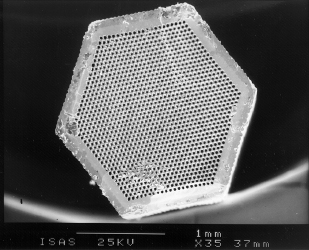
\includegraphics[width = 0.5\textwidth]{bilder/MultiCapillaryColumn}\\
  \caption[Querschnitt einer MCC]{Querschnitt einer MCC \protect\footnotemark}
\end{figure}
\footnotetext{http://yas.yanaco.co.jp/products/import-gc-ims.html}

\section{Peakcharakteristika}
Die im gaschromatographischen Experiment gewonnenen, sowie später auch die simulierten Peaks müssen durch einige Eigenschaften beschrieben werden, um sie vergleichbar zu machen. Dafür seien hier drei solcher Eigenschaften beschrieben, die Lage, Breite und Form eines Peaks.

%Um später die simulierten Peaks mit denen aus den Referenzdatensätzen gut vergleichen zu können, sollen nun einige Eigenschaften aufgeführt werden, die einen Peak beschreiben.

\subsection{Lage}
Die offensichtlichste Eigenschaft eines Peaks ist seine Lage, genauer gesagt, die Lage seines Maximums. Je nach verwendeter Technologie unterscheiden sich die Messzeiträume für einen chomatographischen Durchlauf gewaltig. \todo{Beispielintervalle}
Allerdings gibt es immer einen minimalen Zeitraum der nach Start der Chomatographie vergangen sein muss, bis ein Peak überhaupt auftreten kann. Dieser hängt von der Geschwindigkeit der mobilen Phase ab, da sich die Analyte nicht schneller als die mobile Phase fortbewegen können und daher mindestens dieselbe Zeit benötigen. Außerdem kann für jede einzelne Messung ein Maximalzeitpunkt gewählt werden, nach dem das Experiment beendet wird. 
\todo{Ende der Simulation hier festlegen?}
%Referenzdaten: Manchmal schwierig, wenn die Peaks keine glatte Kurve ergeben, sondern oben zackig sind. 

\subsection{Form}
Außerdem können die Peaks verschiedene Formen haben. Im theoretischen Idealfall haben sie die Form einer Gaußkurve. \todo{Quelle}
Abweichend davon treten in echten Messungen häufig asymmetrische Peaks auf, die dann ein Tailing aufweisen, auch rechtsschiefe genannt. Dabei steigt die Kurve zunächst stark an, sinkt jedoch nach Erreichen des Maximalwerts deutlich langsamer ab, es entsteht ein Schwanz (engl. Tail).
Ursachen für solche schiefen Peaks gibt es viele, einige Beispiele dafür sind zusätzliche Adsorptionseffekte, die beim Altern einer Säule auftreten \cite{kolb2003}, technische Ursachen wie kleinste Hohlräume zwischen der Säule und dem Gaseinlass bzw. -austritt, sowie einige Stoffe, die generell zu Tailing neigen. \todo{Zitat, dass einige Stoffe gererell tailen}. 

Als Maß für die Schiefe bietet sich der Yule-Bowley-Koeffizient an. TODO Formel
\todo{Interquantilskoeffizient, Quelle, Erklären, warum}

\subsection{Breite}
Als drittes können Peaks unterschiedlich breit sein. Da jedoch ein Peak mit größerer Intensität, also möglicherweise größerer Stoffmenge, automatisch auch einen höheren und damit breiteren Peak erzeugt, kann die Halbwertsbreite als Maß für die Peakbreite herangezogen werden. Die Halbwertsbreite wird auf halber Maximalhöhe des Peaks gemessen. Im Fall von auftretendem Tailing ist dieser Wert jedoch wahrscheinlich nicht mehr aussagekräftig. Außerdem ist die Halbwertsbreite kein robustes Maß für die Breite, sodass statt dessen der Interquartilsabstand (IQR) als Maß für die Breite verwendet werden kann. Auch dieses Maß ist unabhängig von der Stoffmenge, die den Peak verursacht hat. 

 Interquartilsabstand 
 \todo{Zitat IQR, diesen erkären, warum dieses Mass}

 
Allgemein ist zu beobachten, dass schnelle Teilchen Peaks zu frühen Zeitpunkten erzeugen, die eine relativ geringe Varianz aufweisen, hingegen spätere Peaks tendenziell breiter werden. Ideale Peaks haben die Form einer Gaußkurve. \todo{Quelle Ideal}

\section{Probabilistische Arithmetische Automaten}
Um die Multikapillarsäule zu simulieren, werden verschiedene Vorgehensweisen angewendet. Am naheliegendsten erscheint es, den chromatographischen Prozess für eine gewisse Anzahl an Teilchen zu simulieren und dabei für jedes einzelne dieser Teilchen mindestens seinen Ort und seinen Zustand festzuhalten. Diese zufallsbasierte Methode hat jedoch den Nachteil, dass verschiedene Durchläufe zu leicht unterschiedlichen Ergebnissen führen können, insbesondere, wenn zu wenige Teilchen simuliert wurden.
Außerdem sind sehr viele teilchen nötig, um glatte Peaks zu bekommen.

Eine andere Möglichkeit besteht darin, die Teilchen als Wahrscheinlichkeitsmasse zu modellieren und für jeden Ort und Zustand festzuhalten, welcher Teil der gesamten Wahrscheinlichkeitsmasse sich dort befindet.
Eine Möglichkeit die Analyte als eine solche Wahrscheinlichkeitsmasse zu betrachten und dadurch eine exakte Verteilung der Teilchen auf Orte und Zustände zu erhalten, bieten Probabilistische Arithmetische Automaten (PAA).
Ein PAA nach \cite{MHKR} ist ein Modell, mit dem eine Folge zufälliger Operationen beschrieben werden kann. 
Für PAA existieren Algorithmen, welche eine gemeinsame Verteilung von Zuständen und Werten oder auch die Verteilung der Wartezeit für einen Wert berechnen. Wie in Kapitel \ref{chapter:mod} beschrieben wird, kann das Modell zur Simulation einer Multikapillarsäule auch als PAA formuliert werden. Mit dieser Formulierung ist die Zeit, die zum Durchlaufen einer Säule gebraucht wird, dann die Wartezeit für den Wert, welcher der Länge der Säule entspricht. %Deshalb kann ein PAA nützlich sein, um neben der eigentlichen Simulation auch noch eine erwartete Verteilung der Ankunftszeiten der Teilchen zu berechnen. 

Zunächst sei hier eine Definition für den PAA gegeben, anschließend wird der Algorithmus zur Berechnung der Wartezeit beschrieben.
%In diesem Fall ist die Länge der Säule der Wert, auf den gewartet wird und man ist interessiert in der Verteilung der Anzahl der Zeitschritte, die benötigt werden, um die Länge zu erreichen. 
%TODO: Wo soll das rein? Sinnvoll, wenn das zu Beginn erklärt
% Was tut ein PAA

\subsection{Definition eines PAA}
% Formale Definition

\begin{definition}[PAA]
 Ein Probabilistischer Arithmetischer Automat (PAA) ist ein Tupel
 $ \mathcal{P} = (\mathcal{Q}, q_0, T, \mathcal{V}, v_0, \mathcal{E}, (e_q)_{q\in\mathcal{Q}}, (\theta_q)_{q\in\mathcal{Q}})$, dabei ist:
 \begin{itemize}
  \item $\mathcal{Q}$ eine endliche Menge von Zuständen
  \item $q_0 \in \mathcal{Q}$ der Startzustand
  \item $T: \mathcal{Q} \times \mathcal{Q} \rightarrow [0,1]$ eine Übergangsfunktion mit $\sum_{q' \in \mathcal{Q}} T(q, q') = 1 $ das heißt $(T(q,q'))_{q,q' \in \mathcal{Q}}$ ist eine stochastische Matrix
  \item $\mathcal{E}$ eine endliche Menge von Emissionen
  \item $e_q: \mathcal{E} \rightarrow [0,1]$ eine Wahrscheinlichkeitsverteilung der Emissionen für jeden Zustand
  \item $\mathcal{V}$ eine Menge von Werten
  \item $v_0$ der Startwert
  \item $\theta_q: \mathcal{V} \times \mathcal{E} \rightarrow \mathcal{V}$ eine Operation für jeden Zustand
 \end{itemize}
\end{definition}
Dabei entspricht $ \mathcal{P} = (\mathcal{Q}, q_0, T)$ einer Markovkette und $ \mathcal{P} = (\mathcal{Q}, q_0, T, \mathcal{E}, (e_q)_{q\in\mathcal{Q}})$ einem Hidden Markov Model. \todo{Muss ich dann Markov erklären?}

Ein PAA ist zu jedem Zeitpunkt mit einer bestimmten Wahrscheinlichkeit in jedem Zustand und kann dabei mit einer bestimmten Wahrscheinlichkeit jeden Wert annehmen. Es existiert also zu jedem Zeitpunkt eine Zustands-Werte-Verteilung. Ausgehend von einer gegebenen Startverteilung, bei dem sich die gesamte Wahrscheinlichkeitsmasse in Zustand $q_0$ befindet und den Wert $v_0$ hat, wird diese Verteilung schrittweise aktualisiert. Dabei findet jeder Übergang gemäß der Wahrscheinlichkeit aus $T$ statt. Wenn sich der Automat mit der Wahrscheinlichkeit $p$ in Zustand $q$ befindet, 
% 
% wahrscheinlichkeit für neuen Zustand $q'$ ausgehend von allen Zuständen $q$
% 
% $ P(q_n'| q_{n-1} ) = (T_{q, q'} \cdot  P(q_{n-1}))$
% 
% $ P(q_n' ) = \sum_q (T_{q, q'} \cdot  P(q_{n-1})$
% Gebe eher p(Q) an

\subsection{Algorithmus zur Berechnung der Wartezeit}
\todo{Algos für die Verteilung und Wartezeit-Berechnung vorstellen}